\documentclass[11pt]{article}

\oddsidemargin=0in
\evensidemargin=0in
\textwidth=6.3in
\topmargin=-0.5in
\textheight=9in

\parindent=0in
%\pagestyle{empty}



%------------------------------------------------------------------
% PROBLEM, PART, AND POINT COUNTING...

% Create the problem number counter.  Initialize to zero.
\newcounter{problemnum}

% Specify that problems should be labeled with arabic numerals.
\renewcommand{\theproblemnum}{\arabic{problemnum}}


% Create the part-within-a-problem counter, "within" the problem counter.
% This counter resets to zero automatically every time the PROBLEMNUM counter
% is incremented.
\newcounter{partnum}[problemnum]

% Specify that parts should be labeled with lowercase letters.
\renewcommand{\thepartnum}{\alph{partnum}}

% Make a counter to keep track of total points assigned to problems...
\newcounter{totalpoints}

% Make counters to keep track of points for parts...
\newcounter{curprobpts}		% Points assigned for the problem as a whole.
\newcounter{totalparts}		% Total points assigned to the various parts.

% Make a counter to keep track of the number of points on each page...
\newcounter{pagepoints}
% This counter is reset each time a page is printed.

% This "program" keeps track of how many points appear on each page, so that
% the total can be printed on the page itself.  Points are added to the total
% for a page when the PART (not the problem) they are assigned to is specified.
% When a problem without parts appears, the PAGEPOINTS are incremented directly
% from the problem as a whole (CURPROBPTS).


%---------------------------------------------------------------------------


% The \problem environment first checks the information about the previous
% problem.  If no parts appeared (or if they were all assigned zero points,
% then it increments TOTALPOINTS directly from CURPROBPTS, the points assigned
% to the last problem as a whole.  If the last problem did contain parts, it
% checks to make sure that their point values total up to the correct sum.
% It then puts the problem number on the page, along with the points assigned
% to it.

\newenvironment{problem}[1]{
% STATEMENTS TO BE EXECUTED WHEN A NEW PROBLEM IS BEGUN:
%
% Increment the problem number counter, and set the current \ref value to that
% number.
\refstepcounter{problemnum}
%
% Add some vspace to separate from the last problem.
\vspace{0.15in} \par
%
\setcounter{curprobpts}{#1} \setcounter{totalparts}{0}	% Reset counters.
%
% Now put in the "announcement" on the page.
{\Large \bf \theproblemnum. \normalsize ({\it \arabic{curprobpts} point\null\ifnum \value{curprobpts} = 1\else s\fi}\/)}
}{
% STATEMENTS TO BE EXECUTED WHEN AN OLD PROBLEM IS ENDED:
%
% If no parts to problem, then increment TOTALPOINTS and PAGEPOINTS for the
% entire problem at once.
\ifnum \value{totalparts} = 0
	\addtocounter{totalpoints}{\value{curprobpts}}	% Add pts to total.
	\addtocounter{pagepoints}{\value{curprobpts}}	% Add pts to page total.
%
% If there were parts for the problem, then check to make sure they total up
% to the same number of points that the problem is worth. Issue a warning
% if not.
\else \ifnum \value{totalparts} = \value{curprobpts}
	\else \typeout{}
	\typeout{!!!!!!!   POINT ACCOUNTING ERROR   !!!!!!!!}
	\typeout{PROBLEM [\theproblemnum] WAS ALLOCATED \arabic{curprobpts} POINTS,}
	\typeout{BUT CONTAINS PARTS TOTALLING \arabic{totalparts} POINTS!}
	\typeout{}
	\fi
\fi
}


%---------------------------------------------------------------------------


% The \newpart command increments the part counter and displays an appropriate
% lowercase letter to mark the part.  It adds points to the point counter
% immediately.  If 0 points are specified, no point announcement is made.
% Otherwise, the announcement is in scriptsize italics.

\newcommand{\newpart}[1]
{
\refstepcounter{partnum}	% Set the current \ref value to the part number.
\hspace{0.25in}		% Indent the part by a quarter inch.
%
% If points are to be printed for this problem (signaled by point value > 0),
% then put them in in scriptsize italics.
\ifnum #1 > 0
	\makebox[0.5in][l]{{\bf \thepartnum.} {\bf ({\it #1 pt\ifnum #1 = 1\else s\fi\/}) \,\,}}
\else
	\makebox[0.25in][l]{({\bf \thepartnum})}
\fi
%
\hspace{0.1in}		% Lead the material away from the part "number".
%
\addtocounter{totalparts}{#1}	% Add points to totalparts for this problem.
\addtocounter{pagepoints}{#1}	% Add points to total for this page.
\addtocounter{totalpoints}{#1}	% Add points to total for entire test.
}


%---------------------------------------------------------------------------



% Just in case you want to skip some numbers in your test...

\newcommand{\skipproblem}[1]{\addtocounter{problemnum}{#1}}



%---------------------------------------------------------------------------


% The \showpoints command simply gives a count of the total points read in up to
% the location at which the command is placed.  Typically, one places one
% \showpoints command at the end of the latex file, just prior to the
% \end{document} command.  It can appear elsewhere, however.

\newcommand{\showpoints}
{
\typeout{}
\typeout{====> A TOTAL OF \arabic{totalpoints} POINTS WERE READ.}
\typeout{}
}


%---------------------------------------------------------------------------



\usepackage{graphicx}
\usepackage[english]{babel}
\usepackage[latin1]{inputenc}
\usepackage{times}
\usepackage[T1]{fontenc}
\usepackage{amsmath}
\usepackage{amssymb}
\usepackage{subfigure}
\usepackage{algorithmic}
\usepackage{algorithm}
\usepackage{url}


\newcommand{\argmax}{\mathop{\arg\max}}
\newcommand{\deriv}[2]{\frac{\partial{#1}}{\partial {#2}} }
\newcommand{\dsep}{\mbox{dsep}}
\newcommand{\Pa}{\mathop{Pa}}
\newcommand{\ND}{\mbox{ND}}
\newcommand{\De}{\mbox{De}}
\newcommand{\Ch}{\mbox{Ch}}
\newcommand{\graphG}{{\mathcal{G}}}
\newcommand{\graphH}{{\mathcal{H}}}
\newcommand{\setA}{\mathcal{A}}
\newcommand{\setB}{\mathcal{B}}
\newcommand{\setS}{\mathcal{S}}
\newcommand{\setV}{\mathcal{V}}
\DeclareMathOperator*{\union}{\bigcup}
\DeclareMathOperator*{\intersection}{\bigcap}
\DeclareMathOperator*{\Val}{Val}
\newcommand{\mbf}[1]{{\mathbf{#1}}}
\newcommand{\eq}{\!=\!}
\newcommand{\cut}[1]{{}}

\begin{document}

%%%(change to appropriate class and semester)
{\centering
  \rule{6.3in}{2pt}
  \vspace{1em}
  \Large{
    CS688: Graphical Models - Spring 2014\\
    Assignment 4\\
  }
  \vspace{1em}
  Assigned: Thursday, Mar 27th. Due: Thursday, April 10th 2:30pm\\
  \vspace{0.1em}
  \rule{6.3in}{1.5pt}
}
\vspace{1pc}

\textbf{General Instructions:} Submit a report with the answers to each question at the start of class on the date the assignment is due. You are encouraged to typeset your solutions. To help you get started, the full \LaTeX source of the assignment is included with the assignment materials. For your assignment to be considered ``on time'', you must upload a zip file containing all of your code to Moodle by the due date. Make sure the code is sufficiently well documented that it's easy to tell what it's doing. You may use any programming language you like. For this assignment, you may \textbf{not} use existing code libraries for inference and learning with CRFs or MRFs. If you think you've found a bug with the data or an error in any of the assignment materials, please post a question to the Moodle discussion forum. Make sure to list in your report any outside references you consulted (books, articles, web pages, etc.) and any students you collaborated with.\\

\textbf{Academic Honesty Statement:} Copying solutions from external sources (books, web pages, etc.) or other students is considered cheating. Sharing your solutions with other students is also considered cheating. Any detected cheating will result in a grade of 0 on the assignment for all students involved, and potentially a grade of F in the course.\\

\textbf{Introduction:} In this assignment, you will experiment with Markov Chain Monte Carlo inference and stochastic maximum likelihood learning for restricted Boltzmann Machines (RBMs). We will use unsupervised feature extraction for handwritten digit recognition as an application domain.\\

\textbf{Data Sets:} We will use binary image data for this assignment taken from the MNIST handwritten digit data set. Examples from this data set are pictured below. Each image has size $28\times 28$.

\begin{figure}[ht]
\centering
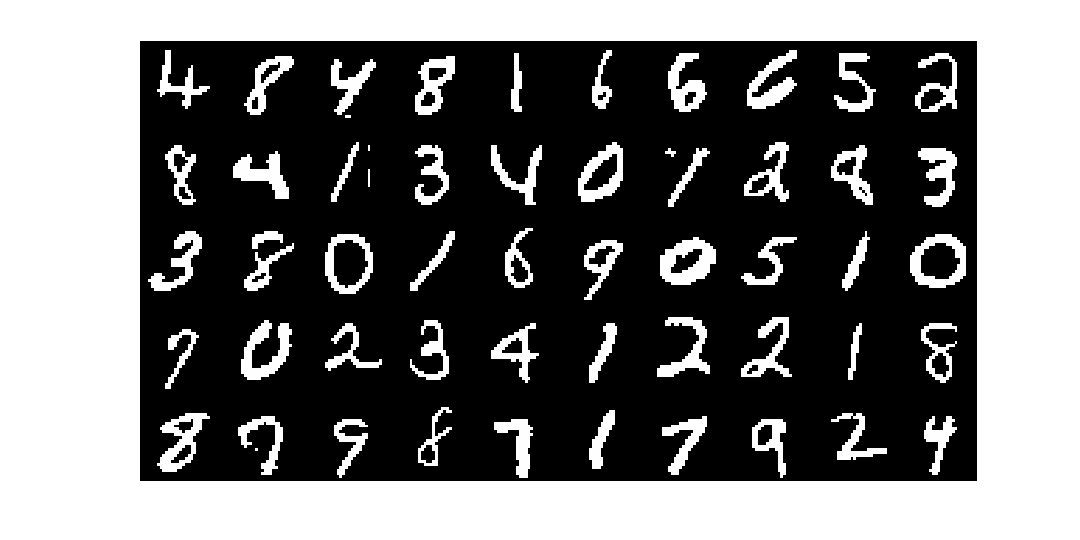
\includegraphics[width=3.1in]{Figures/example_digits.png}
\label{fig_data}
\caption{Example data from the MNIST data set.}
\end{figure}

A model trained on the MNIST data has been provided for use in inference experiments.  The MNIST data set contains 
binary images stored as row vectors.
The training image file \textit{MNISTXtrain.txt} contains $60,000$ rows and the test image file \textit{MNISTXtest.txt} contains $10,000$ rows. Each row of the file contains one $28\times 28$ binary image stored as a $784$ element vector in row-major format. The MNIST data set also contains labels indicating the class of each image. The class labels go from $1$ to $10$ and correspond to the digits $0$ to $9$. The $60,000$ training image labels are stored in the file \textit{MNISTYtrain.txt}. The $10,000$ test labels are stored in the file \textit{MNISTYtest.txt}.\\

\textbf{Graphical Model: } We will consider modeling this data using a binary restricted Boltzmann machine model, pictured below. The RBM is a Markov network model with two layers of variables $\mbf{X}$ and $\mbf{H}$. The $\mbf{X}$ variables $X_1,...,X_D$ constitute the first layer of the model and are referred to as the \textit{visible variables} or \textit{visible units}. The second layer of the model consists of the $\mbf{H}$ variables $H_1,...,H_K$ referred to as the \textit{hidden variables} or \textit{hidden units}. The Markov network structure underlying the RBM is a bipartite graph where there are edges between the visible units and the hidden units, but not within the hidden units or within the visible units. \\

\begin{figure}[ht]
\centering
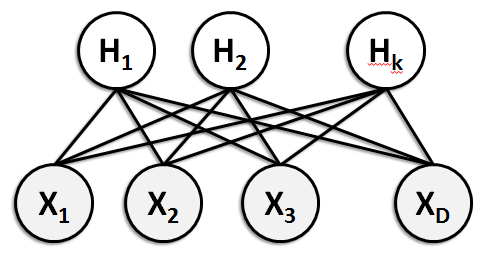
\includegraphics[width=2.5in]{Figures/rbm.png}
\caption{RBM Graphical Model}
\end{figure}

In the context of learning models for images, the $\mbf{X}$ variables represent the binary pixels of the image. It is more convenient to consider each image as a length $D=784$ vector for use with this model, which is how they are stored in the data files. The hidden units are also a binary vector of length $K$. When $K$ is less than $D$, we can view the hidden units as a lower-dimensional encoding of the image. We can think of learning the RBM model parameters roughly as learning to extract features that can be used to encode the visible units with minimal loss of information. This encoding can be used for a variety of tasks including classification, which we will explore later in the assignment.\\

\textbf{Probabilistic Model:} The probabilistic model underlying the RBM is essentially the same as that underlying the Ising model and the CRF model. The main difference is that in the RBM, the hidden variables are never observed. The model can be defined through a joint energy function on the hidden and visible variables as seen below. The model parameters $W^P_{dk}$ encode the
pairwise compatibility between $x_d$ and $h_k$. The model parameters $W^B_k$ and $W^C_d$
provide a bias that either encourages or discourages $h_k$ and $x_d$ from turning on.

\begin{align}
\label{energy}
E_W(\mbf{x},\mbf{h})&=
-\sum_{d=1}^D\sum_{k=1}^K W^P_{dk}x_dh_k - \sum_{k=1}^KW^B_k h_k - \sum_{d=1}^D W^C_d x_d
\end{align}

Using the standard log-linear mapping between energies and probabilities, we obtain the joint distribution over the visible and hidden variables as follows. Like the Ising model and CRF, the partition function of the RBM is a sum over all configurations of all the variables in the model.

\begin{align}
\label{joint-prob}
P_W(\mbf{X}=\mbf{x},\mbf{H}=\mbf{h})&= \frac{\exp(-E_W(\mbf{x},\mbf{h}))}
{\sum_{\mbf{x}'}\sum_{\mbf{h}'}\exp(-E_W(\mbf{x}',\mbf{h}'))}
\end{align}

Since the hidden variables are never observed, when we learn the model parameters we must marginalize away the hidden variables and optimize the log likelihood of the parameters given the values of the visible variables only. The marginal probability of the visible variables is given below.

\begin{align}
\label{marginal-prob}
P_W(\mbf{X}=\mbf{x})&= \sum_{\mbf{h}}P_W(\mbf{X}=\mbf{x},\mbf{H}=\mbf{h}) \\
&=\frac{\sum_{\mbf{h}}\exp(-E_W(\mbf{x},\mbf{h}))}
{\sum_{\mbf{x}'}\sum_{\mbf{h}'}\exp(-E_W(\mbf{x}',\mbf{h}'))}
\end{align}


\textbf{Inference Algorithm:} One of the main benefits of RBM models relative to other models is that inference for the visible variables given the hidden variables and inference for the hidden variables given the visible variables is very easy due to the structure of the graph. In particular, given all of the $\mbf{X}$ variables, all of the $\mbf{H}$ variables are independent of each other since there are no connections within the hidden layer. By symmetry, the $\mbf{X}$ variables are all independent of each other given the $\mbf{H}$ variables. This gives us a very simple block-Gibbs algorithm for drawing samples from an RBM. The algorithm alternates between sampling each visible unit independently of the other visible units conditioned on all of the hidden units and sampling each hidden unit independently of the other hidden units given the values for the visible units. The required conditional probabilities are given below.

\begin{align}
\label{pxgh}
P_W(X_d=x_d|\mbf{h})&= \frac{\exp(W^C_dx_d + \sum_{k=1}^K W^P_{dk}x_dh_k)}
{1+ \exp(W^C_d + \sum_{k=1}^K W^P_{dk}h_k) }\\
\label{phgx}
P_W(H_k=h_k|\mbf{x})&= \frac{\exp(W^B_kh_k + \sum_{d=1}^D W^P_{dk}x_dh_k )}
{1+ \exp(W^B_k + \sum_{d=1}^D W^P_{dk}x_d + ) }
\end{align}

The complete block Gibbs sampling algorithm for the RBM is listed below. Recall that to draw a sample $z$ from a distribution $P(Z)$ over a binary random variable $Z$, we first draw a random number $u$ from a uniform distribution on $[0,1]$. We set $z=1$ if $u<P(Z=1)$ and $z=0$ otherwise. Combined with the conditional distributions listed above, this is all you need to implement the block Gibbs sampler given RBM parameters $W^P$,$W^B$ and $W^C$.\\

\begin{algorithm}[h!]
\begin{algorithmic}
\STATE $RBMBlockGibbsSample(W^P,W^B,W^C,S)$
\STATE \textbf{for} $k$ from $1$ to $K$ Initialize $h_k^0$ to a random binary value
\FOR{$s$ from $1$ to $S$}
\STATE \textbf{for} $d$ from $1$ to $D$ Sample $x_d^{s}\sim P_W(X_d=x_d|\mbf{h}^{s-1})$
\STATE \textbf{for} $k$ from $1$ to $K$ Sample $h_k^{s}\sim P_W(H_k=h_k|\mbf{x}^{s})$
\ENDFOR
\STATE Return $\mbf{x}^1,...,\mbf{x}^S$ and $\mbf{h}^1,...,\mbf{h}^S$
\end{algorithmic}
\caption{Block Gibbs Sampler for the RBM model}
\label{inference}
\end{algorithm}
\medskip

\textbf{Learning Algorithm:} To learn the model, we require the gradients of the average log marginal likelihood. We form the average log marginal likelihood below, and list it's gradients with respect to $W_{ij}^P$ and $W^B_j$ and $W^C_i$

\begin{align}
\label{marginal_loglik}
\mathcal{L}(W|\mbf{x}_{1:N})&=\frac{1}{N}\sum_{n=1}^N\log(P_W(\mbf{X}=\mbf{x}_n))\\
%
\label{deriv_WP}
\deriv{\mathcal{L}(W|\mbf{x}_{1:N})}{W^P_{ij}}
&= \left(\frac{1}{N}\sum_{n=1}^Nx_{ni}P_W(H_j=1|\mbf{X}=\mbf{x}_n)\right)
-P_W(X_i=1,H_j=1)\\
%
\label{deriv_WB}
\deriv{\mathcal{L}(W|\mbf{x}_{1:N})}{W^B_{j}}
&= \left(\frac{1}{N}\sum_{n=1}^NP_W(H_j=1|\mbf{X}=\mbf{x}_n)\right)
-P_W(H_j=1)\\
%
\label{deriv_WC}
\deriv{\mathcal{L}(W|\mbf{x}_{1:N})}{W^C_{i}}
&= \left(\frac{1}{N}\sum_{n=1}^Nx_{ni}\right) -P_W(X_i=1)
\end{align}

The gradient for each parameter has the form of a difference of two terms. We call the first term, which depends on the data, the positive term, and the second term, which is independent of the data, the negative term. Due to the partition function, the average log marginal likelihood itself can not be tractably computed. While the positive term in each of the gradients can be computed exactly using the inference formula for hidden variables, the negative term in the gradients involves a marginal probability that can not be tractably computed and requires approximation.\\

Given a collection of samples $\tilde{\mbf{x}}_{1:S}$ drawn from $P_W(\mbf{X},\mbf{H})$, we can form a stochastic approximation to the gradients as seen below. Note that we could also use samples for $H_j$ to approximate the gradient, but this would unnecessarily introduce additional noise since we can exactly represent the conditional distribution $P_W(H_j=1|\mbf{X}=\tilde{\mbf{x}}_s)$.

\begin{align}
\label{deriv_approx_WP}
\deriv{\mathcal{L}(W|\mbf{x}_{1:N})}{W^P_{ij}}
&\approx \left(\frac{1}{N}\sum_{n=1}^Nx_{ni}P_W(H_j=1|\mbf{X}=\mbf{x}_n)\right)
-\left(\frac{1}{S}\sum_{s=1}^S\tilde{x}_{si}P_W(H_j=1|\mbf{X}=\tilde{\mbf{x}}_s)\right)\\
%
\label{deriv_approx_WB}
\deriv{\mathcal{L}(W|\mbf{x}_{1:N})}{W^B_{j}}
&\approx \left(\frac{1}{N}\sum_{n=1}^NP_W(H_j=1|\mbf{X}=\mbf{x}_n)\right)
-\left(\frac{1}{S}\sum_{s=1}^SP_W(H_j=1|\mbf{X}=\tilde{\mbf{x}}_s)\right)\\
%
\label{deriv_approx_WC}
\deriv{\mathcal{L}(W|\mbf{x}_{1:N})}{W^C_{i}}
&\approx \left(\frac{1}{N}\sum_{n=1}^N x_{ni}\right)
-\left(\frac{1}{S}\sum_{s=1}^S \tilde{x}_{si}\right)
\end{align}

Given a stochastic approximation to the gradients, we can then take a step in the gradient direction to update the parameters. This requires the selection of a step size $\alpha$.

\begin{align}
\label{update_WP}
W^P_{ij} \leftarrow W^P_{ij} + \alpha \deriv{\mathcal{L}(W|\mbf{x}_{1:N})}{W^P_{ij}}\\
\label{update_WB}
W^B_{j} \leftarrow W^B_{j} + \alpha \deriv{\mathcal{L}(W|\mbf{x}_{1:N})}{W^B_{j}}\\
\label{update_WC}
W^C_{i} \leftarrow W^C_{i} + \alpha \deriv{\mathcal{L}(W|\mbf{x}_{1:N})}{W^C_{i}}
\end{align}

We now have all the components in place that are needed to learn the model. We will apply the stochastic
maximum likelihood algorithm. We interleave the block Gibbs updates needed to compute the negative contribution to the gradient with the parameter updates. We run $C$ parallel chains during learning. On each iteration of the algorithm, we compute the positive contribution to the gradients, compute the negative contribution to the gradients using the current sample from each of the $C$ chains, update the current samples from each of the $C$ chains using one step of block Gibbs, and then take a step in the gradient direction.\\

There are two other modifications that help the learning algorithm  to converge faster and give better results. The first modification is to break the data up into a set of $B$ batches and to update the model parameters after processing the data in each batch. This is called mini-batch stochastic descent. The second modification is to add regularization to the parameters to prevent over-fitting during training. This requires the introduction of a regularization parameter $\lambda$.\\

Detailed pseudo code for the complete mini-batch stochastic ascent learning algorithm for binary RBMs is given below. We use $T$ to indicate the number of learning iterations, $B$ to indicate the number of batches, $N_B$ to indicate the number of data cases in each batch, and $C$ to indicate the number of chains. We use the vectors $\tilde{\mbf{x}}_c$ and $\tilde{\mbf{h}}_c$ to store the states of each of the $C$ chains. We use $\alpha$ to indicate the step size for the gradient descent procedure and $\lambda$ to indicate the strength of the regularizer.

\begin{algorithm}
\begin{algorithmic}
\STATE $RBMLearn(\mbf{x}_{1:N},T,B,C,K,\alpha,\lambda)$
\STATE \#Initialize the Gibbs chains
\FOR{$c$ from $1$ to $C$}
\STATE \textbf{for} $k$ from $1$ to $K$ \textbf{do} Initialize $\tilde{h}_{ck}$ to a random binary value \textbf{end}
\ENDFOR
\STATE \#Initialize the parameters
\STATE \textbf{for} $k$ from $1$ to $K$ \textbf{do} Initialize $W^B_{k} \sim \mathcal{N}(0,0.1^2)$ \textbf{end}
\STATE \textbf{for} $d$ from $1$ to $D$ \textbf{do} Initialize $W^C_{d} \sim \mathcal{N}(0,0.1^2)$ \textbf{end}
\FOR{$k$ from $1$ to $K$}
\STATE \textbf{for} $d$ from $1$ to $D$ \textbf{do} Initialize $W^P_{dk} \sim \mathcal{N}(0,0.1^2)$ \textbf{end}
\ENDFOR
\FOR{$t$ from $1$ to $T$}
  \FOR{$b$ from $1$ to $B$}
    \STATE \#Compute positive gradient contribution from each data case in batch b
    \STATE $gWC^+ \leftarrow 0, gWB^+ \leftarrow 0, gWP^+\leftarrow 0$
    \FOR{$n$ from $1+(b-1)N_B$ to $bN_B$}
      \STATE  \textbf{for} $d$ from $1$ to $D$ \textbf{do} $gWC_{d}^+ \leftarrow gWC_{d}^+ + x_{nd}$ \textbf{end}
      \FOR{$k$ from $1$ to $K$}
        \STATE  $p_k \leftarrow P_W(H_k=1|\mbf{X}=\mbf{x}_n)$
        \STATE  $gWB_{k}^+ \leftarrow gWB_{k}^+ + p_k$
        \STATE  \textbf{for} $d$ from $1$ to $D$ \textbf{do} $gWP_{dk}^+ \leftarrow gWP_{dk}^+ + x_{nd}p_k$ \textbf{end}
      \ENDFOR
    \ENDFOR
    \STATE \#Compute negative gradient contribution from each chain and sample states
    \STATE $gWC^- \leftarrow 0, gWB^- \leftarrow 0, gWP^-\leftarrow 0$
    \FOR{$c$ from $1$ to $C$}
      \STATE \textbf{for} $d$ from $1$ to $D$ \textbf{do} $\tilde{x}_{cd} \sim P_W(X_d|\mbf{H}=\tilde{\mbf{h}}_c)$ \textbf{end}
      \STATE \textbf{for} $k$ from $1$ to $K$ \textbf{do} $\tilde{h}_{ck} \sim P_W(H_k|\mbf{X}=\tilde{\mbf{x}}_c)$ \textbf{end}
      \STATE  \textbf{for} $d$ from $1$ to $D$ \textbf{do} $gWC_{d}^- \leftarrow gWC_{d}^- + \tilde{x}_{cd}$ \textbf{end}
      \FOR{$k$ from $1$ to $K$}
        \STATE  $p_k \leftarrow P_W(H_k=1|\mbf{X}=\tilde{\mbf{x}}_c)$
        \STATE  $gWB_{k}^- \leftarrow gWB_{k}^- + p_k$
        \STATE  \textbf{for} $d$ from $1$ to $D$ \textbf{do}
            $gWP_{dk}^- \leftarrow gWP_{dk}^- + \tilde{x}_{cd}p_k$ \textbf{end}
      \ENDFOR
    \ENDFOR
      \STATE \#Take a gradient step for each parameter in the model
      \STATE   \textbf{for} $d$ from $1$ to $D$ \textbf{do}  $W^C_d \leftarrow W^C_d +  \alpha\left(\frac{gWC_{d}^+}{N_B} - 
               \frac{gWC_{d}^-}{C} -\lambda W^C_d\right)$ \textbf{end}
      \FOR{$k$ from $1$ to $K$}
        \STATE  $W^B_k \leftarrow W^B_k +  \alpha\left(\frac{gWB_{k}^+}{N_B} - \frac{gWB_{k}^-}{C} -\lambda W^B_k\right)$
        \STATE   \textbf{for} $d$ from $1$ to $D$ \textbf{do}  $W^P_{dk} \leftarrow W^P_{dk} +  \alpha\left(\frac{gWP_{dk}^+}{N_B} - \frac{gWP_{dk}^-}{C} -\lambda W^P_{dk}\right)$ \textbf{end}
      \ENDFOR
  \ENDFOR
\ENDFOR
\STATE Return $W^P,W^B,W^C$
\end{algorithmic}
\caption{Mini-batch stochastic gradient ascent for the RBM model}
\label{learning}
\end{algorithm}



\begin{problem}{20} \textbf{Derivations:} Perform the following derivations. Show your work.\\

\textbf{(a)} Starting from the definition of the joint probability on $\mbf{X}$ and $\mbf{H}$ given in Equation \ref{joint-prob}, derive the conditional probability  $P_W(X_d=x_d|\mbf{h})$ shown in Equation \ref{pxgh}. \textbf{Hint:} You can do this from first principles, but it will be easier if you use the factor reduction algorithm.\\

\textbf{(b)} Starting from the definition of the average marginal log likelihood in Equation \ref{marginal_loglik}, derive the partial derivative of the average marginal log likelihood with respect to $W^P_{ij}$ shown in Equation \ref{deriv_WP}. \textbf{Hint:} This derivation is very similar to both the Ising model and CRF model maximum likelihood parameter estimation derivations.
\end{problem}

\begin{problem}{20} \textbf{Inference, Burn-In and Autocorrelation:} Implement the block Gibbs sampler described in Algorithm 1. In the models directory, you will find the files \textit{MNISTWP.txt}, \textit{MNISTWB.txt} and \textit{MNISTWC.txt}. These files contain the parameters of a binary RBM model trained on the MNIST data set using $K=100$ hidden units. \textit{MNISTWP.txt} contains the learned $W^P$ parameters as a $100\times 784$ matrix (space-separated). \textit{MNISTWB.txt} contains the learned $W^B$ parameters as a $1\times 100$ vector (space separated). \textit{MNISTWC.txt} contains the learned $W^C$ parameters as a $1\times 784$ vector (space separated). Use your implementation of the Block Gibbs sampler and these trained parameters to answer the following questions.\\

\textbf{(a)} Run your sampling implementation on the trained MNIST model for $500$ iterations starting from a random binary hidden vector. Display every 5th sample of the visible variables as a $28 \times 28$ image and include these images in your report (there is Matlab/Octave helper code for assembling the
individual images into a single large image in the Code/Images directory). How similar do the samples look compared to the example training data shown in Figure \ref{fig_data}? Describe any differences. How similar are the samples to each other? 

\textbf{(b)} Use your implementation to run $100$ separate chains (initialized to different random binary hidden vectors) for $500$ iterations each. Display the final sample of the visible variables from each of the $100$ chains as a $28 \times 28$ image and include the images in your report. How similar are the samples from the different chains? 

\textbf{(c)} For the first $5$ of the $100$ chains run in part (b), compute the energy of each sample of the visible and hidden variables $(\mbf{x}_{s},\mbf{h}_{s})$ using Equation \ref{energy}. Plot a single graph with $5$ curves showing the energy trace for each chain versus the sampling iteration. Do the energies of the samples from the different chains converge to similar values? What can we conclude about the burn-in and autocorrelation times for the Gibbs sampler applied to this model?
\end{problem}

\begin{problem}{30} \textbf{Learning:} Implement the mini batch stochastic gradient ascent algorithm for RBM learning shown in Algorithm 2 and use your implementation to answer the following questions.\\

\textbf{(a)} Run your learning algorithm on the MNIST training data. Use $T=50$ training iterations, $K=400$ hidden units, $B=100$ batches of $N_B=600$ data cases at a time, $C=100$ Gibbs chains, a step size of $\alpha=0.1$ and regularization parameter $\lambda=0.0001$. When training is complete, display the final sample from each of the $100$ Gibbs chains as a $28\times 28$ image. Include the image of the samples in your report. How similar do the samples look compared to the example MNIST training images shown in Figure 1? How do they compare to the samples produced by the $K=100$ model used in Question 2?.\\

\textbf{(b)} The $W^P$ parameters associated with each hidden unit $k$ also form a $784$-long vector which can be visualized as a $28 \times 28$ image. This image can be interpreted as the ``receptive field" of the hidden unit. It indicates how much the different pixels in the input image contribute to the probability of activating the hidden unit. Display the receptive field images for each of the $400$ hidden units. Comment on any structure (or lack of structure) you see in the receptive fields.
\end{problem}

\begin{problem}{30} \textbf{Feature Extraction and Classification:} Using your model trained on MNIST, convert each data case $\mbf{x}_n$ into the lower dimensional vector $\mbf{z}_n$ given by $\mbf{z}_{nk} = P_W(H_k=1|\mbf{X}=\mbf{x}_n)$. We will use these lower dimensional vectors as feature vectors for digit classification with a multi-class support vector machine classifier (\url{http://svmlight.joachims.org/svm_multiclass.html}). SVMmulticlass uses a simple, sparse ascii file format called the SVMlight format. The SVMlight format contains one data case per line. The format of line $n$ is: $y_n$ $1:z_{n1}$ $2:z_{n2}$ ... $K:z_{nK}$. If a particular feature $z_{nk}$ is zero (or sufficiently close to zero) you can skip over the $k:z_{nk}$ entry in the file (there is helper Matlab/Octave code for writing SVMlight format files in the Code/SVM directory). Use your extracted features and the SVMmulticlass software to answer the following questions.\\

\textbf{(a)} Write out a classification training file in SVMlight format using the labels for the training digits and the lower-dimensional feature vectors $\mbf{z}_n$ for the training digits. Also write out a classification test file in SVM-light format using the labels for the test digits and the lower-dimensional feature vectors $\mbf{z}_n$ for the test digits. Run the SVMmulticlass classification code included in the Code/SVM directory on your training data file and use the trained model to classify the test cases. Report the error rate your model achieves as a percentage. The commands needed to run the SVMmulticlass code for training and testing are:\\

\begin{verbatim}
svm_multiclass_learn -c 1000000 -v 2 -e 1 <train_data_file> <model_file>
svm_multiclass_classify -v 2 <test_data_file> <model_file> <predictions>
\end{verbatim}

\textbf{(b)} Re-run the svm training experiment from part (a) using the raw pixel values instead of the lower-dimensional representation extracted using the RBM. Report the error rate achieved using the raw pixel values as a percentage. Which features work better for classification?

\end{problem}

\showpoints
\end{document} 